\documentclass[border=5mm]{standalone}
\usepackage{tikz}
\usepackage{siunitx}
\usepackage{bm}
\usepackage{caption}
\usetikzlibrary{patterns, arrows.meta}

% Définition des couleurs
\definecolor{pmma}{RGB}{255, 200, 150}
\definecolor{water}{RGB}{100, 180, 255}
\definecolor{tungsten}{RGB}{80, 80, 80}
\definecolor{preplane}{RGB}{255, 140, 0}
\definecolor{postplane}{RGB}{148, 0, 211}
\definecolor{wpetg}{RGB}{180, 180, 190}
\definecolor{Carnelian}{RGB}{179, 27, 27}

\begin{document}
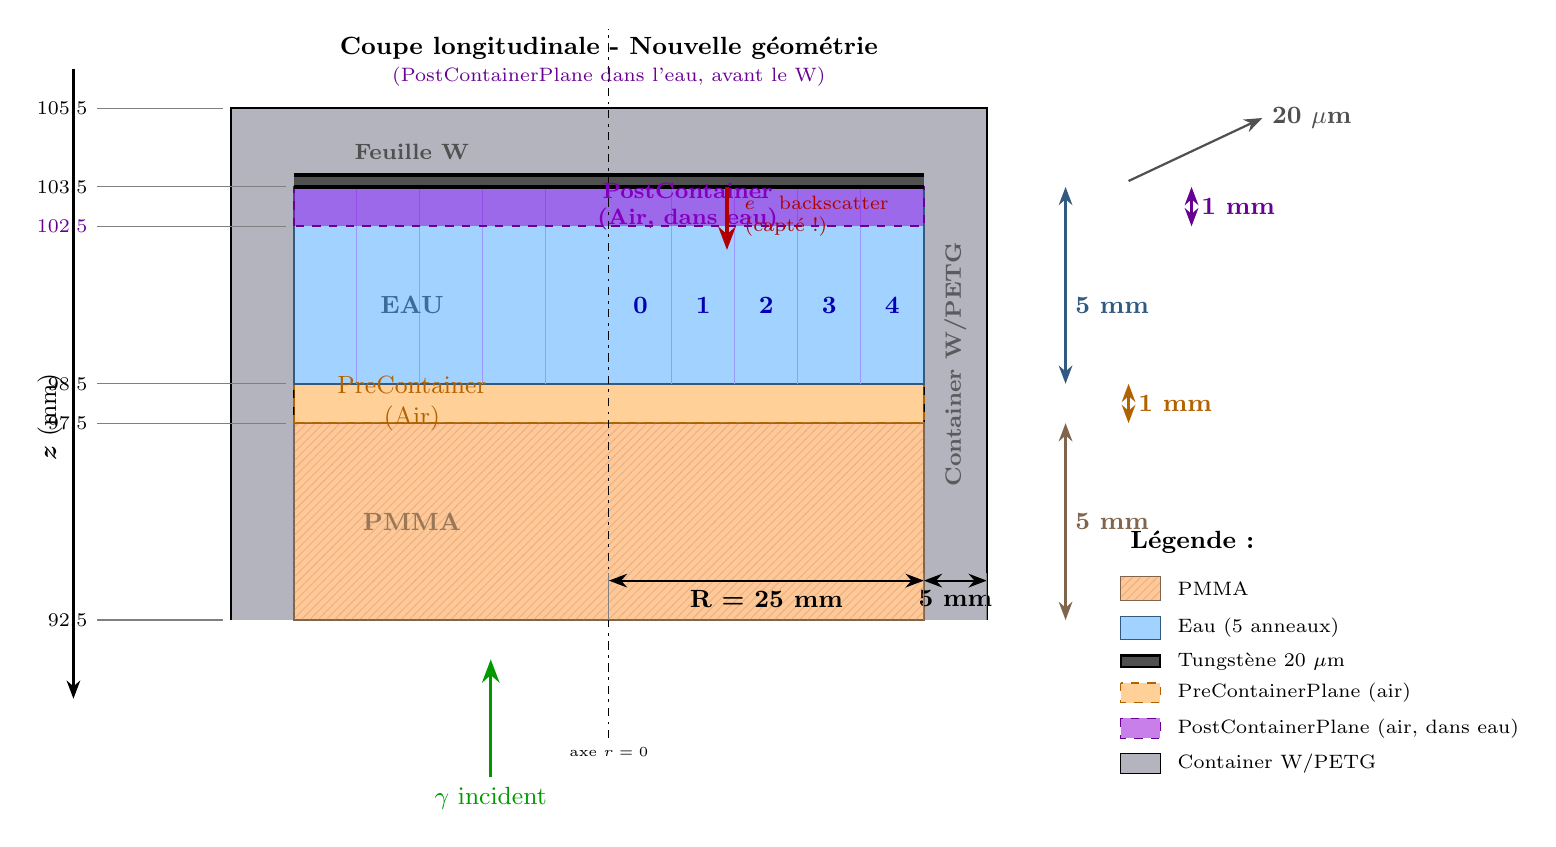
\begin{tikzpicture}[>=Stealth, font=\small]

    % ═══════════════════════════════════════════════════════════════════════
    % ÉCHELLE : 1 unité TikZ = 1 mm
    % Facteur d'échelle horizontal (r) : 0.16
    % Facteur d'échelle vertical (z) : 0.5
    % ═══════════════════════════════════════════════════════════════════════
    
    \def\scaleR{0.16}
    \def\scaleZ{0.5}
    
    % ═══════════════════════════════════════════════════════════════════════
    % NOUVELLE GÉOMÉTRIE (PostContainerPlane DANS l'eau, AVANT le W)
    % ═══════════════════════════════════════════════════════════════════════
    
    % Positions z (en mm)
    \def\zPMMAbot{92.5}
    \def\zPMMAtop{97.5}
    \def\zPreBot{97.5}
    \def\zPreTop{98.5}
    \def\zWaterBot{98.5}
    \def\zWaterTop{103.5}
    % MODIFIÉ : PostContainerPlane maintenant DANS l'eau (102.5 - 103.5 mm)
    \def\zPostBot{102.5}
    \def\zPostTop{103.5}
    % Feuille de tungstène juste après le haut de l'eau/PostContainer
    \def\zTungstenBot{103.5}
    \def\zTungstenTop{103.52}
    \def\zContainerBot{103.5}
    \def\zContainerTop{105.5}
    
    % Rayons (en mm)
    \def\Rinner{25}
    \def\Router{30}
    
    % Décalage pour centrer
    \def\zoff{-98}
    
    % ═══════════════════════════════════════════════════════════════════════
    % DESSIN DES ÉLÉMENTS (de bas en haut)
    % ═══════════════════════════════════════════════════════════════════════
    
    % --- Parois du container (W/PETG) ---
    \fill[wpetg] ({-\Router*\scaleR}, {(\zPMMAbot+\zoff)*\scaleZ}) rectangle ({-\Rinner*\scaleR}, {(\zContainerTop+\zoff)*\scaleZ});
    \fill[wpetg] ({\Rinner*\scaleR}, {(\zPMMAbot+\zoff)*\scaleZ}) rectangle ({\Router*\scaleR}, {(\zContainerTop+\zoff)*\scaleZ});
    % Fond du container
    \fill[wpetg] ({-\Router*\scaleR}, {(\zContainerBot+\zoff)*\scaleZ}) rectangle ({\Router*\scaleR}, {(\zContainerTop+\zoff)*\scaleZ});
    
    % Contours container
    \draw[black, thick] ({-\Router*\scaleR}, {(\zPMMAbot+\zoff)*\scaleZ}) -- ({-\Router*\scaleR}, {(\zContainerTop+\zoff)*\scaleZ}) -- ({\Router*\scaleR}, {(\zContainerTop+\zoff)*\scaleZ}) -- ({\Router*\scaleR}, {(\zPMMAbot+\zoff)*\scaleZ});
    \draw[black, thick] ({-\Rinner*\scaleR}, {(\zPMMAbot+\zoff)*\scaleZ}) -- ({-\Rinner*\scaleR}, {(\zContainerBot+\zoff)*\scaleZ}) -- ({\Rinner*\scaleR}, {(\zContainerBot+\zoff)*\scaleZ}) -- ({\Rinner*\scaleR}, {(\zPMMAbot+\zoff)*\scaleZ});
    
    % --- PMMA (5 mm) ---
    \fill[pmma] ({-\Rinner*\scaleR}, {(\zPMMAbot+\zoff)*\scaleZ}) rectangle ({\Rinner*\scaleR}, {(\zPMMAtop+\zoff)*\scaleZ});
    \draw[pmma!50!black, thick] ({-\Rinner*\scaleR}, {(\zPMMAbot+\zoff)*\scaleZ}) rectangle ({\Rinner*\scaleR}, {(\zPMMAtop+\zoff)*\scaleZ});
    % Hachures PMMA
    \fill[pattern=north east lines, pattern color=pmma!70!black, opacity=0.3] ({-\Rinner*\scaleR}, {(\zPMMAbot+\zoff)*\scaleZ}) rectangle ({\Rinner*\scaleR}, {(\zPMMAtop+\zoff)*\scaleZ});
    
    % --- PreContainerPlane (1 mm, air) ---
    \fill[preplane, opacity=0.4] ({-\Rinner*\scaleR}, {(\zPreBot+\zoff)*\scaleZ}) rectangle ({\Rinner*\scaleR}, {(\zPreTop+\zoff)*\scaleZ});
    \draw[preplane!70!black, thick, dashed] ({-\Rinner*\scaleR}, {(\zPreBot+\zoff)*\scaleZ}) rectangle ({\Rinner*\scaleR}, {(\zPreTop+\zoff)*\scaleZ});
    
    % --- Eau (5 mm, 5 anneaux) ---
    \fill[water, opacity=0.6] ({-\Rinner*\scaleR}, {(\zWaterBot+\zoff)*\scaleZ}) rectangle ({\Rinner*\scaleR}, {(\zWaterTop+\zoff)*\scaleZ});
    \draw[water!50!black, thick] ({-\Rinner*\scaleR}, {(\zWaterBot+\zoff)*\scaleZ}) rectangle ({\Rinner*\scaleR}, {(\zWaterTop+\zoff)*\scaleZ});
    % Limites des anneaux
    \foreach \r in {5, 10, 15, 20} {
        \draw[blue!40, thin] ({-\r*\scaleR}, {(\zWaterBot+\zoff)*\scaleZ}) -- ({-\r*\scaleR}, {(\zWaterTop+\zoff)*\scaleZ});
        \draw[blue!40, thin] ({\r*\scaleR}, {(\zWaterBot+\zoff)*\scaleZ}) -- ({\r*\scaleR}, {(\zWaterTop+\zoff)*\scaleZ});
    }
    % Labels anneaux
    \node[font=\small, blue!70!black] at ({2.5*\scaleR}, {(100.5+\zoff)*\scaleZ}) {\textbf{0}};
    \node[font=\small, blue!70!black] at ({7.5*\scaleR}, {(100.5+\zoff)*\scaleZ}) {\textbf{1}};
    \node[font=\small, blue!70!black] at ({12.5*\scaleR}, {(100.5+\zoff)*\scaleZ}) {\textbf{2}};
    \node[font=\small, blue!70!black] at ({17.5*\scaleR}, {(100.5+\zoff)*\scaleZ}) {\textbf{3}};
    \node[font=\small, blue!70!black] at ({22.5*\scaleR}, {(100.5+\zoff)*\scaleZ}) {\textbf{4}};
    
    % --- PostContainerPlane (1 mm, AIR) - MAINTENANT DANS L'EAU ---
    \fill[postplane, opacity=0.5] ({-\Rinner*\scaleR}, {(\zPostBot+\zoff)*\scaleZ}) rectangle ({\Rinner*\scaleR}, {(\zPostTop+\zoff)*\scaleZ});
    \draw[postplane!70!black, thick, dashed] ({-\Rinner*\scaleR}, {(\zPostBot+\zoff)*\scaleZ}) rectangle ({\Rinner*\scaleR}, {(\zPostTop+\zoff)*\scaleZ});
    
    % --- Feuille de Tungstène (20 µm) - épaisseur exagérée pour visibilité ---
    \def\Wthick{0.15}  % Épaisseur visuelle exagérée
    \fill[tungsten] ({-\Rinner*\scaleR}, {(\zTungstenBot+\zoff)*\scaleZ}) rectangle ({\Rinner*\scaleR}, {(\zTungstenBot+\zoff)*\scaleZ + \Wthick});
    \draw[black, very thick] ({-\Rinner*\scaleR}, {(\zTungstenBot+\zoff)*\scaleZ}) -- ({\Rinner*\scaleR}, {(\zTungstenBot+\zoff)*\scaleZ});
    \draw[black, very thick] ({-\Rinner*\scaleR}, {(\zTungstenBot+\zoff)*\scaleZ + \Wthick}) -- ({\Rinner*\scaleR}, {(\zTungstenBot+\zoff)*\scaleZ + \Wthick});
    
    % ═══════════════════════════════════════════════════════════════════════
    % AXE DE SYMÉTRIE
    % ═══════════════════════════════════════════════════════════════════════
    
    \draw[black, dash pattern=on 3pt off 2pt on 1pt off 2pt, thin] (0, {(\zPMMAbot+\zoff-3)*\scaleZ}) -- (0, {(\zContainerTop+\zoff+2)*\scaleZ});
    \node[below, font=\tiny] at (0, {(\zPMMAbot+\zoff-3)*\scaleZ}) {axe $r=0$};
    
    % ═══════════════════════════════════════════════════════════════════════
    % COTES VERTICALES (positions z) - À GAUCHE
    % ═══════════════════════════════════════════════════════════════════════
    
    \def\cotex{-6.5}
    
    % Ligne de référence
    \draw[gray, thin] ({\cotex}, {(\zPMMAbot+\zoff)*\scaleZ}) -- ({-\Router*\scaleR-0.1}, {(\zPMMAbot+\zoff)*\scaleZ});
    \draw[gray, thin] ({\cotex}, {(\zPMMAtop+\zoff)*\scaleZ}) -- ({-\Rinner*\scaleR-0.1}, {(\zPMMAtop+\zoff)*\scaleZ});
    \draw[gray, thin] ({\cotex}, {(\zPreTop+\zoff)*\scaleZ}) -- ({-\Rinner*\scaleR-0.1}, {(\zPreTop+\zoff)*\scaleZ});
    \draw[gray, thin] ({\cotex}, {(\zPostBot+\zoff)*\scaleZ}) -- ({-\Rinner*\scaleR-0.1}, {(\zPostBot+\zoff)*\scaleZ});
    \draw[gray, thin] ({\cotex}, {(\zWaterTop+\zoff)*\scaleZ}) -- ({-\Rinner*\scaleR-0.1}, {(\zWaterTop+\zoff)*\scaleZ});
    \draw[gray, thin] ({\cotex}, {(\zContainerTop+\zoff)*\scaleZ}) -- ({-\Router*\scaleR-0.1}, {(\zContainerTop+\zoff)*\scaleZ});
    
    % Valeurs z
    \node[left, font=\scriptsize] at ({\cotex}, {(\zPMMAbot+\zoff)*\scaleZ}) {92.5};
    \node[left, font=\scriptsize] at ({\cotex}, {(\zPMMAtop+\zoff)*\scaleZ}) {97.5};
    \node[left, font=\scriptsize] at ({\cotex}, {(\zPreTop+\zoff)*\scaleZ}) {98.5};
    \node[left, font=\scriptsize, postplane!70!black] at ({\cotex}, {(\zPostBot+\zoff)*\scaleZ}) {102.5};
    \node[left, font=\scriptsize] at ({\cotex}, {(\zWaterTop+\zoff)*\scaleZ}) {103.5};
    \node[left, font=\scriptsize] at ({\cotex}, {(\zContainerTop+\zoff)*\scaleZ}) {105.5};
    
    % Label axe z
    \draw[<-, thick] ({\cotex-0.3}, {(\zPMMAbot+\zoff-2)*\scaleZ}) -- ({\cotex-0.3}, {(\zContainerTop+\zoff+1)*\scaleZ});
    \node[left, font=\small, rotate=90] at ({\cotex-0.6}, {(99+\zoff)*\scaleZ}) {$\bm{z}$ (mm)};
    
    % ═══════════════════════════════════════════════════════════════════════
    % COTES DES ÉPAISSEURS - À DROITE
    % ═══════════════════════════════════════════════════════════════════════
    
    \def\cotexR{5.8}
    
    % PMMA : 5 mm
    \draw[<->, thick, pmma!50!black] ({\cotexR}, {(\zPMMAbot+\zoff)*\scaleZ}) -- ({\cotexR}, {(\zPMMAtop+\zoff)*\scaleZ});
    \node[right, font=\small, pmma!50!black] at ({\cotexR}, {(95+\zoff)*\scaleZ}) {\textbf{5 mm}};
    
    % PreContainerPlane : 1 mm
    \draw[<->, thick, preplane!70!black] ({\cotexR+0.8}, {(\zPreBot+\zoff)*\scaleZ}) -- ({\cotexR+0.8}, {(\zPreTop+\zoff)*\scaleZ});
    \node[right, font=\small, preplane!70!black] at ({\cotexR+0.8}, {(98+\zoff)*\scaleZ}) {\textbf{1 mm}};
    
    % Eau : 5 mm
    \draw[<->, thick, water!50!black] ({\cotexR}, {(\zWaterBot+\zoff)*\scaleZ}) -- ({\cotexR}, {(\zWaterTop+\zoff)*\scaleZ});
    \node[right, font=\small, water!50!black] at ({\cotexR}, {(100.5+\zoff)*\scaleZ}) {\textbf{5 mm}};
    
    % PostContainerPlane : 1 mm (DANS L'EAU)
    \draw[<->, thick, postplane!70!black] ({\cotexR+1.6}, {(\zPostBot+\zoff)*\scaleZ}) -- ({\cotexR+1.6}, {(\zPostTop+\zoff)*\scaleZ});
    \node[right, font=\small, postplane!70!black] at ({\cotexR+1.6}, {(103+\zoff)*\scaleZ}) {\textbf{1 mm}};
    
    % Tungstène : 20 µm (avec flèche vers zoom)
    \draw[->, thick, tungsten] ({\cotexR+0.8}, {(\zTungstenBot+\zoff)*\scaleZ + \Wthick/2}) -- ({\cotexR+2.5}, {(\zTungstenBot+\zoff)*\scaleZ + \Wthick/2 + 0.8});
    \node[right, font=\small, tungsten] at ({\cotexR+2.5}, {(\zTungstenBot+\zoff)*\scaleZ + \Wthick/2 + 0.8}) {\textbf{20 $\mu$m}};
    
    % ═══════════════════════════════════════════════════════════════════════
    % COTES HORIZONTALES (rayons) - EN BAS
    % ═══════════════════════════════════════════════════════════════════════
    
    \def\cotey{-4.5}
    
    % R = 25 mm
    \draw[<->, thick] (0, {\cotey*\scaleZ}) -- ({\Rinner*\scaleR}, {\cotey*\scaleZ});
    \node[below, font=\small] at ({12.5*\scaleR}, {\cotey*\scaleZ}) {\textbf{R = 25 mm}};
    
    % Paroi = 5 mm
    \draw[<->, thick] ({\Rinner*\scaleR}, {\cotey*\scaleZ}) -- ({\Router*\scaleR}, {\cotey*\scaleZ});
    \node[below, font=\small] at ({27.5*\scaleR}, {\cotey*\scaleZ}) {\textbf{5 mm}};
    
    % Lignes de rappel
    \draw[gray, thin] (0, {(\zPMMAbot+\zoff)*\scaleZ}) -- (0, {\cotey*\scaleZ + 0.1});
    \draw[gray, thin] ({\Rinner*\scaleR}, {(\zPMMAbot+\zoff)*\scaleZ}) -- ({\Rinner*\scaleR}, {\cotey*\scaleZ + 0.1});
    \draw[gray, thin] ({\Router*\scaleR}, {(\zPMMAbot+\zoff)*\scaleZ}) -- ({\Router*\scaleR}, {\cotey*\scaleZ + 0.1});
    
    % ═══════════════════════════════════════════════════════════════════════
    % LABELS DES MATÉRIAUX
    % ═══════════════════════════════════════════════════════════════════════
    
    \def\labelx{-2.5}
    
    % PMMA
    \node[font=\small\bfseries, pmma!60!black] at ({\labelx}, {(95+\zoff)*\scaleZ}) {\textbf{PMMA}};
    
    % PreContainerPlane
    \node[font=\small, preplane!70!black, align=center] at ({\labelx}, {(98+\zoff)*\scaleZ}) {PreContainer\\(Air)};
    
    % Eau
    \node[font=\small\bfseries, water!60!black] at ({\labelx}, {(100.5+\zoff)*\scaleZ}) {\textbf{EAU}};
    
    % PostContainerPlane (DANS L'EAU)
    \node[font=\footnotesize\bfseries, postplane!90!black, align=center] at ({\labelx+3.5}, {(103+\zoff)*\scaleZ}) {PostContainer\\(Air, dans eau)};
    
    % Tungstène
    \node[font=\footnotesize\bfseries, tungsten] at ({\labelx}, {(103.5+\zoff)*\scaleZ + \Wthick + 0.3}) {\textbf{Feuille W}};
    
    % Container
    \node[font=\footnotesize, wpetg!50!black, rotate=90] at ({(\Rinner+2.5)*\scaleR}, {(99+\zoff)*\scaleZ}) {\textbf{Container W/PETG}};
    
    % ═══════════════════════════════════════════════════════════════════════
    % FLÈCHES POUR LE BACKSCATTER
    % ═══════════════════════════════════════════════════════════════════════
    
    % Flèche photon incident
    \draw[->, very thick, green!60!black] (-1.5, {(\zPMMAbot+\zoff-4)*\scaleZ}) -- (-1.5, {(\zPMMAbot+\zoff-1)*\scaleZ});
    \node[below, font=\small, green!60!black] at (-1.5, {(\zPMMAbot+\zoff-4)*\scaleZ}) {$\gamma$ incident};
    
    % Flèche électron backscatter du W (vers -z)
    \draw[->, very thick, red!70!black] (1.5, {(\zTungstenBot+\zoff)*\scaleZ}) -- (1.5, {(\zPostBot+\zoff)*\scaleZ - 0.3});
    \node[right, font=\scriptsize, red!70!black, align=left] at (1.6, {(102.8+\zoff)*\scaleZ}) {$e^-$ backscatter\\(capté !)};
    
    % ═══════════════════════════════════════════════════════════════════════
    % TITRE
    % ═══════════════════════════════════════════════════════════════════════
    
    \node[above, font=\small\bfseries] at (0, {(\zContainerTop+\zoff+1)*\scaleZ}) {Coupe longitudinale - Nouvelle géométrie};
    \node[above, font=\scriptsize, postplane!70!black] at (0, {(\zContainerTop+\zoff+0.3)*\scaleZ}) {(PostContainerPlane dans l'eau, avant le W)};
    
    % ═══════════════════════════════════════════════════════════════════════
    % LÉGENDE
    % ═══════════════════════════════════════════════════════════════════════
    
    \def\legx{6.5}
    \def\legy{-1.5}
    
    \node[anchor=north west, font=\small\bfseries] at ({\legx}, {\legy}) {Légende :};
    
    % Espacement vertical entre les éléments de la légende
    \def\legspacing{0.45}
    \def\legstart{0.7}
    
    % PMMA
    \def\ypmma{\legy-\legstart}
    \fill[pmma] ({\legx}, {\ypmma}) rectangle ({\legx+0.5}, {\ypmma-0.3});
    \fill[pattern=north east lines, pattern color=pmma!70!black, opacity=0.3] ({\legx}, {\ypmma}) rectangle ({\legx+0.5}, {\ypmma-0.3});
    \draw[pmma!50!black] ({\legx}, {\ypmma}) rectangle ({\legx+0.5}, {\ypmma-0.3});
    \node[right, font=\scriptsize] at ({\legx+0.6}, {\ypmma-0.15}) {PMMA};
    
    % Eau
    \def\yeau{\legy-\legstart-0.5}
    \fill[water, opacity=0.6] ({\legx}, {\yeau}) rectangle ({\legx+0.5}, {\yeau-0.3});
    \draw[water!50!black] ({\legx}, {\yeau}) rectangle ({\legx+0.5}, {\yeau-0.3});
    \node[right, font=\scriptsize] at ({\legx+0.6}, {\yeau-0.15}) {Eau (5 anneaux)};
    
    % Tungstène
    \def\ytung{\legy-\legstart-1.0}
    \fill[tungsten] ({\legx}, {\ytung}) rectangle ({\legx+0.5}, {\ytung-0.15});
    \draw[black, thick] ({\legx}, {\ytung}) rectangle ({\legx+0.5}, {\ytung-0.15});
    \node[right, font=\scriptsize] at ({\legx+0.6}, {\ytung-0.075}) {Tungstène 20 $\mu$m};
    
    % PreContainerPlane
    \def\ypre{\legy-\legstart-1.35}
    \fill[preplane, opacity=0.4] ({\legx}, {\ypre}) rectangle ({\legx+0.5}, {\ypre-0.25});
    \draw[preplane!70!black, dashed] ({\legx}, {\ypre}) rectangle ({\legx+0.5}, {\ypre-0.25});
    \node[right, font=\scriptsize] at ({\legx+0.6}, {\ypre-0.125}) {PreContainerPlane (air)};
    
    % PostContainerPlane - MODIFIÉ
    \def\ypost{\legy-\legstart-1.8}
    \fill[postplane, opacity=0.5] ({\legx}, {\ypost}) rectangle ({\legx+0.5}, {\ypost-0.25});
    \draw[postplane!70!black, dashed] ({\legx}, {\ypost}) rectangle ({\legx+0.5}, {\ypost-0.25});
    \node[right, font=\scriptsize] at ({\legx+0.6}, {\ypost-0.125}) {PostContainerPlane (air, dans eau)};
    
    % Container
    \def\ycont{\legy-\legstart-2.25}
    \fill[wpetg] ({\legx}, {\ycont}) rectangle ({\legx+0.5}, {\ycont-0.25});
    \draw[black] ({\legx}, {\ycont}) rectangle ({\legx+0.5}, {\ycont-0.25});
    \node[right, font=\scriptsize] at ({\legx+0.6}, {\ycont-0.125}) {Container W/PETG};

\end{tikzpicture}
\end{document}
